\documentclass[12pt,letterpaper]{article}
\usepackage[utf8]{inputenc}
\usepackage[spanish]{babel}
\usepackage{amsmath}
\usepackage{amsfonts}
\usepackage{amssymb}
\usepackage{graphicx}
\usepackage[left=2cm,right=2cm,top=2cm,bottom=2cm]{geometry}
\author{Oscar Daniel Rosario Morales,Israel Hipolito Mejia 
Alba}

\title{Practica N 11 "INTRODUCCIÓN A OpenMP" 
EDA 2}
\begin{document}
\maketitle
Grupo: 8 


Profesor : Tista Garcia Edgar

\newpage
\subsection{Objetivo:}
El estudiante conocerá y aprenderá a utilizar algunas de las directivas de OpenMP utilizadas para realizar programas paralelos.

\subsection{Actividades:}
* Revisar el ambiente necesario para trabajar con OpenMP y el lenguaje C.

* Realizar ejemplos del funcionamiento de las primeras directivas de OpenMP en el lenguaje C.

* Realizar un primer programa que se resuelva un programa de forma paralela utilizando las directivas de OpenMP.

\subsection{Desarrollo}
\subsubsection*{Actividad 1} 
En un editor de texto teclear el siguiente código y guardarlo con extension ".c", por ejemplo hola.c. Después desde la consola o linea de comandos de linux, situarse en el directorio donde se encuentra el código fuente y compilarlo de la siguiente manera.


\begin{flushleft}
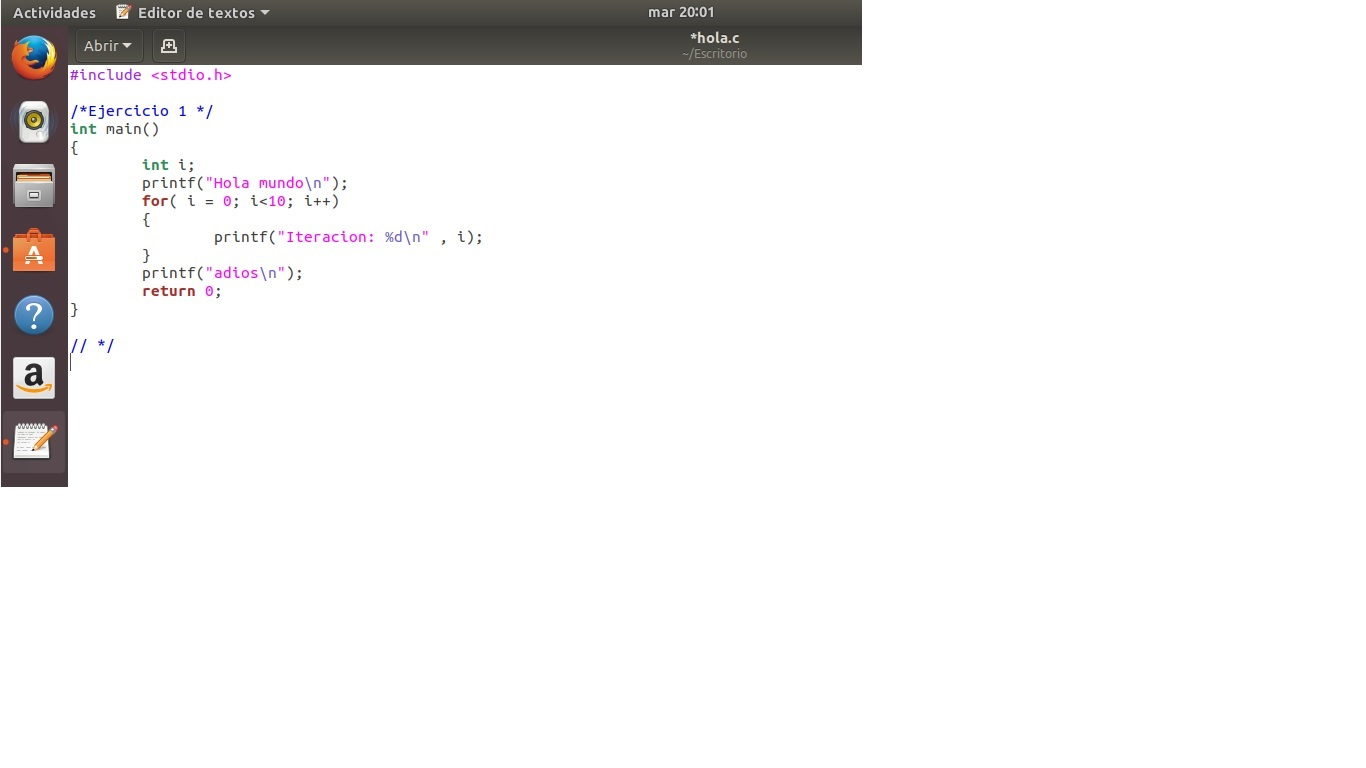
\includegraphics[scale=1]{ejercicio0.jpg} 

\end{flushleft}

\begin{flushleft}
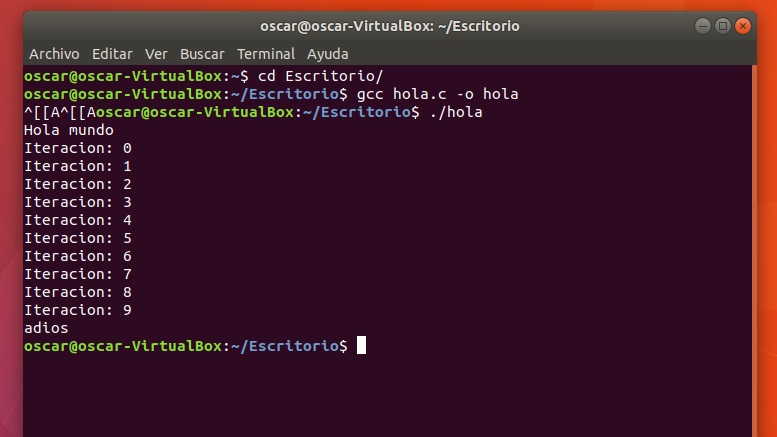
\includegraphics[scale=.8]{ejercicio01.jpg} 

\end{flushleft}

Una vez que ya se tiene el código en su version serial, se formara una región paralela. Entonces agregar al código anterior el constructor \textbf{parallel} desde la declaración de la variable hasta antes de la ultima impresion de pantalla, como se muestra.
Para compilarlo hay que indicar que se agregaran las directivas de openMP, lo que se realiza agregando la bandera en la compilación -fopenmp.

\begin{flushleft}
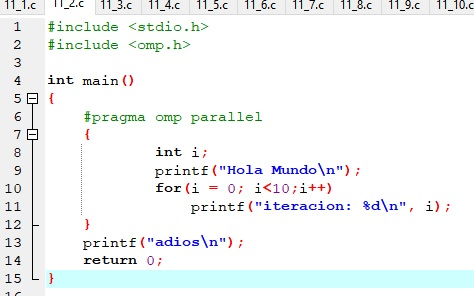
\includegraphics[scale=.8]{ejercicio1.jpg} 

\end{flushleft}

\begin{flushleft}
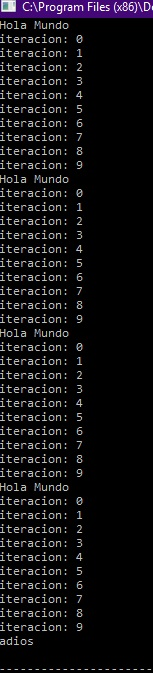
\includegraphics[scale=.8]{ejercicio11.jpg} 

\end{flushleft}




¿Qué diferencia hay en la salida del programa con respecto al secuencial?
En el programa paralelo , se repitió el proceso de imprimir las iteraciones. 

¿Por qué se obtiene esa salida?
Esto se debe a que se ejecuta el proceso en diversos hilos. Aunque cabe mencionar que no siempre da la misma salida, en algunos casos, al realizar la impresión del hola mundo, no se imprimen las iteraciones y se agregan a otro proceso, repitiendo las iteraciones en uno de los casos.
\subsubsection*{Actividad 2}

Cambia el numero de hilos que habáa en la región paralela a un numero n ( entero) probar cada una de las formas indicadas.
\begin{flushleft}
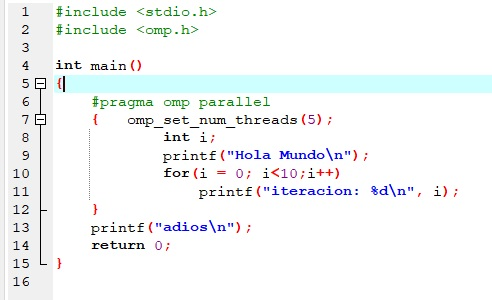
\includegraphics[scale=.8]{ejercicio2.jpg} 

\end{flushleft}

\begin{flushleft}
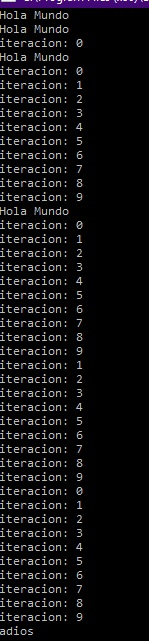
\includegraphics[scale=.8]{ejercicio21.jpg} 

\end{flushleft}
\begin{flushleft}
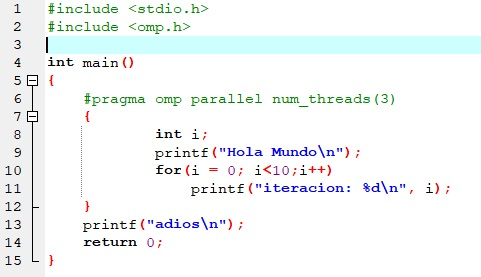
\includegraphics[scale=.8]{ejercicio22.jpg} 

\end{flushleft}

\begin{flushleft}
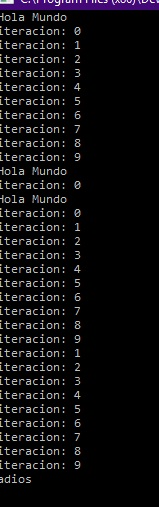
\includegraphics[scale=.8]{ejercicio23.jpg} 

\end{flushleft}


¿Qué sucedió en la ejecución con respecto a la actividad 1? En el primer caso donde se cambia el numero de hilos a través de la función omp set num threads(n =5), se puede observar que las iteraciones muchas de ellas se repiten en un proceso, y en otros solo se realizo una impresión de hola mundo. 
En el segundo caso donde se agrego la clausula en el constructor parallel no n= 3, se puede observar que paso lo mismo sin embargo solo se obtuvieron 3 hola mundo y en una proceso se repiten las iteraciones.



\subsubsection*{Actividad 3}

Del codigo que se esta trabajando, sacar de la region paralela la declaracion de la variable int , compilar y ejecutar varias veces.
\begin{flushleft}
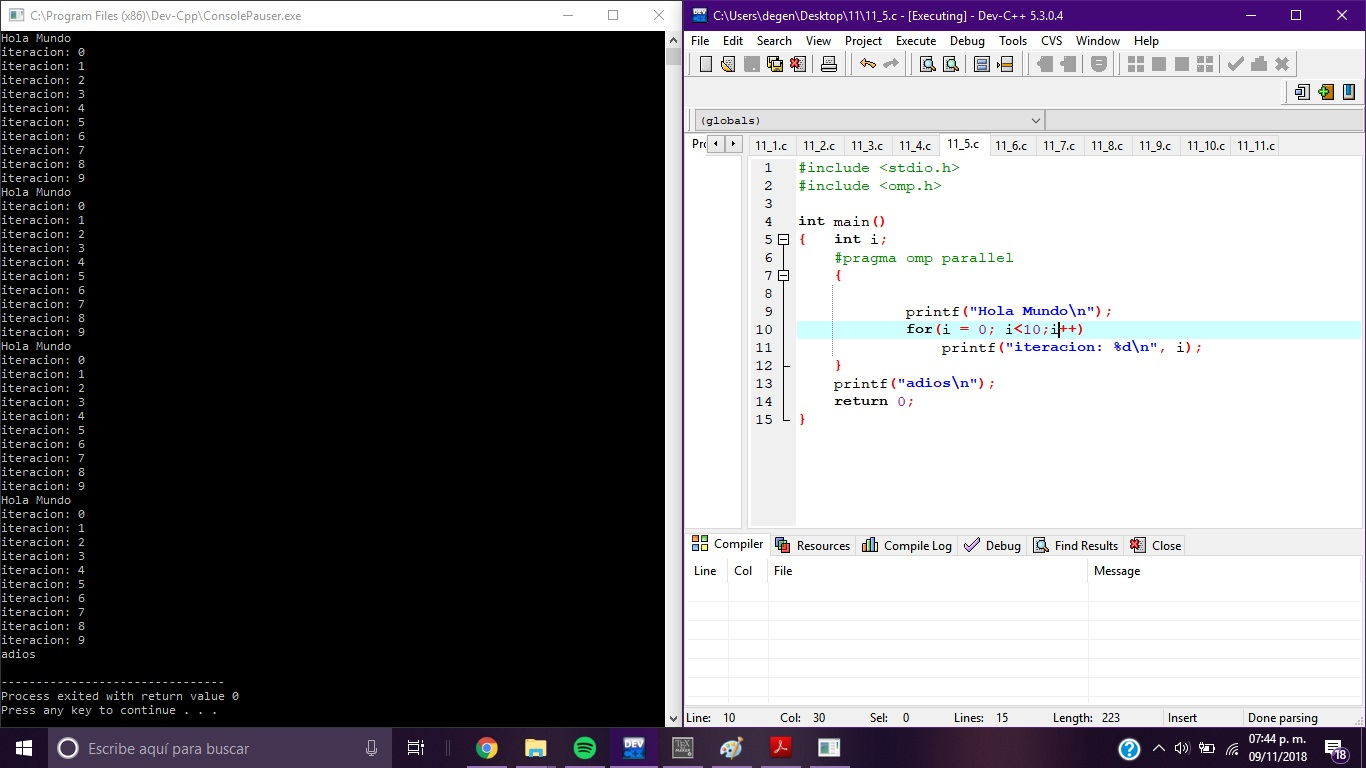
\includegraphics[scale=.5]{ejercicio3.jpg} 

\end{flushleft}

\begin{flushleft}
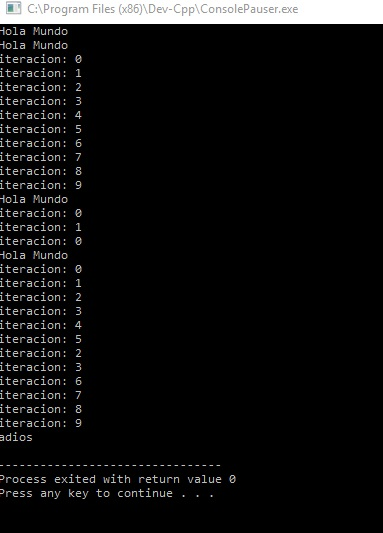
\includegraphics[scale=.8]{ejercicio31.jpg} 

\end{flushleft}
¿Qué sucedió y por qué? En la primera imagen se puede observar que las iteraciones se ejecutan correctamente, aunque el proceso se repite 4 veces, esto se debe a que la variable que se utilizara en el ciclo for se hizo publica de la paralelización, se sitúa fuera del bloque a paralelizar, esto quiere decir que es una variable que sera compartida en memoria entre los hilos, al estar dentro la variable cada proceso la utilizaba de manera individual.




\subsubsection*{Actividad 4}
Existen dos cláusulas que pueden forzar que una variable privada sea compartida y una compartida sea privada. 
Al código resultante de la actividad 3, agregar la cláusula \textit{private()}  después del constructor parallel, con la variable i dentro.
\begin{flushleft}
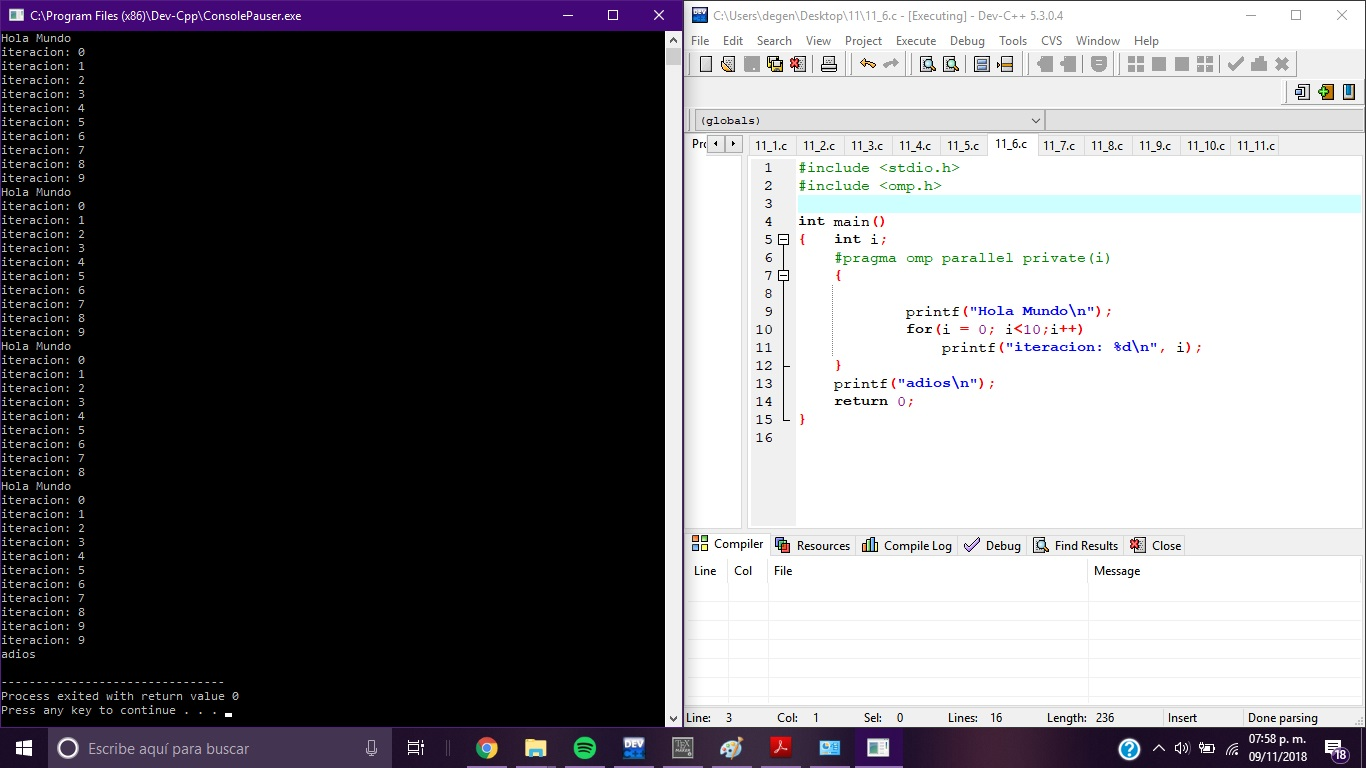
\includegraphics[scale=.5]{ejercicio4.jpg} 

\end{flushleft}

¿Qué sucedió? Se puede observar que de nuevo, se realizaron las iteraciones correspondientes a cada hilo , lo que sucedió fue que la variable i paso de ser compartida a privada por lo que crearon copias, una para cada hilo, la cual sera utilizada durante el proceso del hilo y al final serán eliminadas.

\subsubsection*{Actividad 5}
Dentro de la region paralela hay un número de hilos generados y cada uno tiene asignado un identificador. Estos datos se pueden conocer durante la ejecución con la llamada a las funciones de la biblioteca \textit{omp.get.num.threads()} y \textit{omp.get.trhread.num()} respectivamente.
Probar el siguiente ejemplo y notar que para su buen funcionamiento se debe indicar que la variable tid sea privada dentro de la región paralela, ya que de no ser así todos los hilos escribirán en la dirección de memoria asignada a dicha variable sin un control \textit{( race condition)}, es decir \textit{"competiran"} para ver quien llega antes y el resultado visualizado puede ser inconsistente e impredecible.

\begin{flushleft}
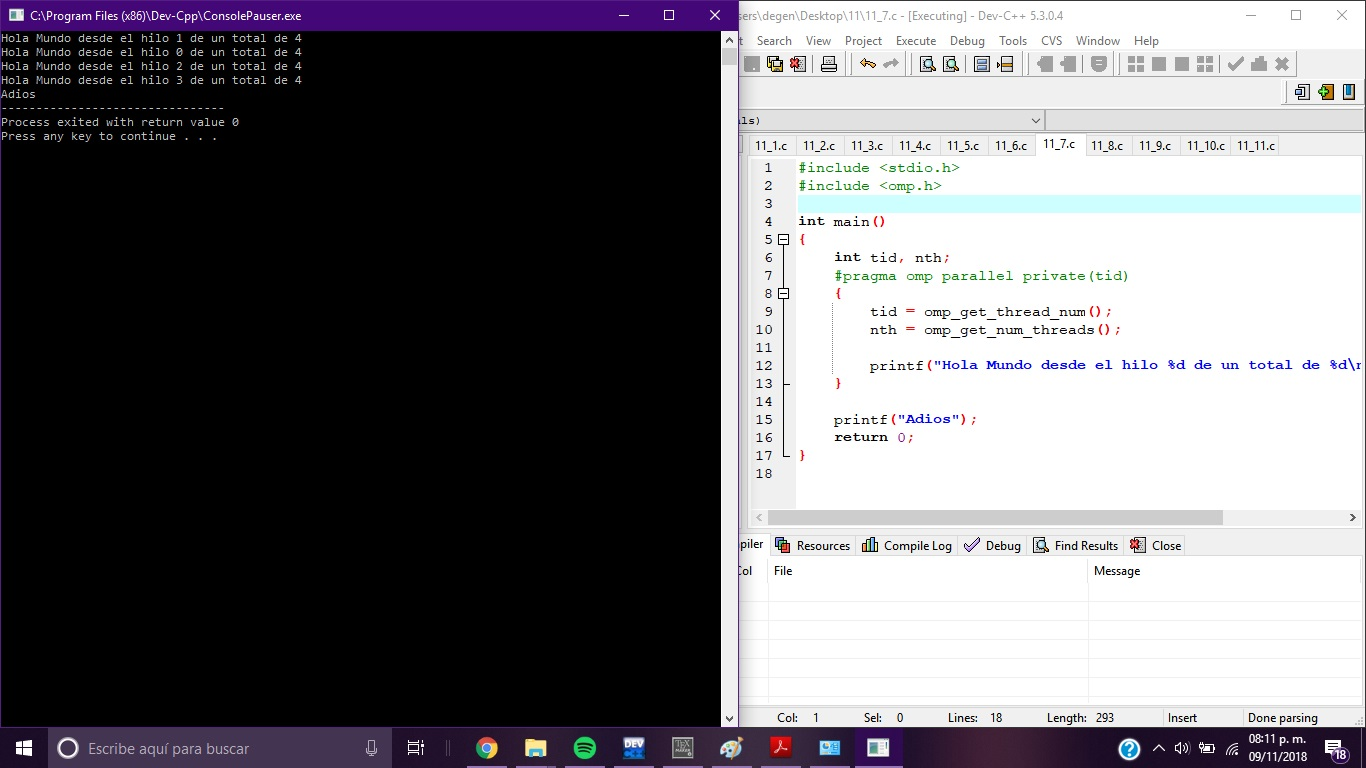
\includegraphics[scale=.5]{ejercicio5.jpg} 

\end{flushleft}

Probar el ejemplo quitando del código la clasula private para visualizar el comportamiento del programa.


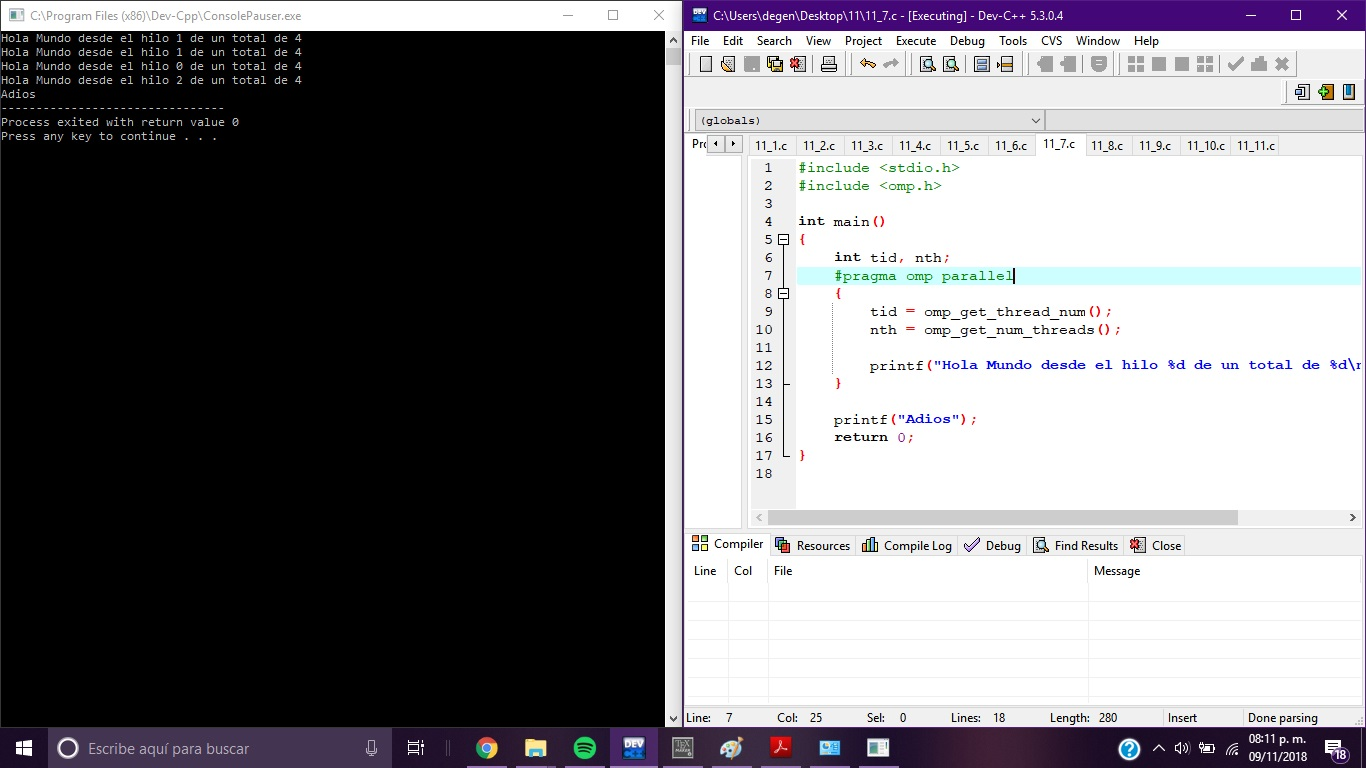
\includegraphics[scale=.5]{ejercicio51.jpg}
¿Qué sucedió? Como se comentaba anteriormente al mantener la variable tid como compartida, se sobre escriben los datos ya que se utilizan repetidas veces, tal como se ve la impresión de identificación del hilo 1/4 se repite una vez. 


\subsubsection*{Actividad 6}
Se requiere realizar la suma de dos arreglos unidimensionales de 10 elementos de forma paralela utilizando solo dos hilos. Para ello se utilizará un paralelismo de datos o descomposición de dominio, es decir, cada hilo trabajará con diferentes elementos de los arreglos a sumar A y B, pero ambos utilizarán el mismo algoritmo para realizar la suma.

Realizar programa en su version serial.

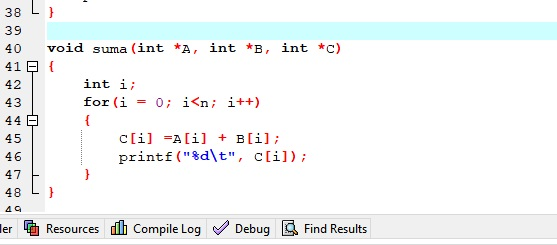
\includegraphics[scale=.8]{ejercicio6.jpg}


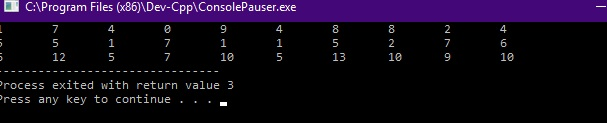
\includegraphics[scale=1]{ejercicio61.jpg}

Para la version paralela, el hilo 0 sumará la primera mitad de A con la primera mitad de B y el hilo 1 sumará las segundas mitades. Para conseguir esto cada hilo realizará las mismas instrucciones, pero utilizará indices diferentes para referirse a diferentes elementos de los arreglos, cada uno iniciará y terminará el indice i en valores distintos.

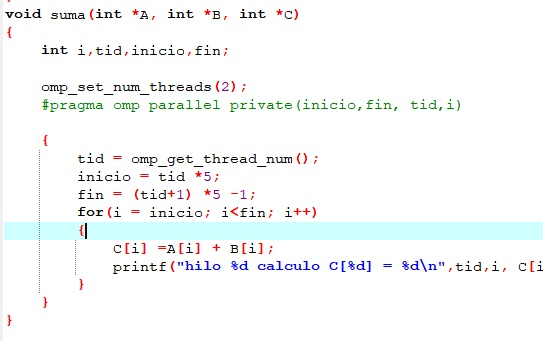
\includegraphics[scale=.8]{ejercicio62.jpg}


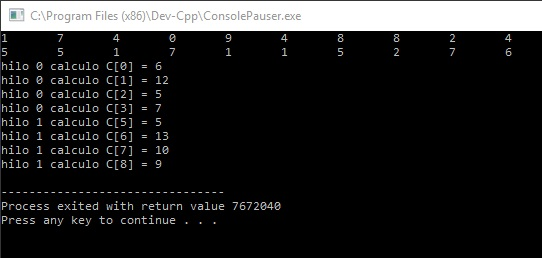
\includegraphics[scale=1]{ejercicio63.jpg}


Lo que se cambio fue que los intervalos para cada for que se realizaba en un hilo fueron diferentes, como solo iban a hacer 2 hilos, se tendría el hilo 0 y el hilo 1, para el primer hilo , su for va desde i = 0, hasta i = 4, y en el segundo hilo va desde i = 5 ,hasta i = 9 , así se recorre el entero de tamaño 10 por completo pero cada hilo realizando las mismas operaciones en su mitad perteneciente.

\subsubsection*{Actividad 7}

Otro constructor es el for, el cual divide las iteraciones de una estructura de repetición for. Para utilizarlo se debe estar dentro de una región paralela.
Lo que realiza este constructor es que la variable de control que se utiliza para iterar se hará automáticamente privada, esto es para que cada hilo trabaje con su propia variable i.

Modifica el código de la actividad 1, de manera que se dividan las iteraciones de la estructura de repetición for.

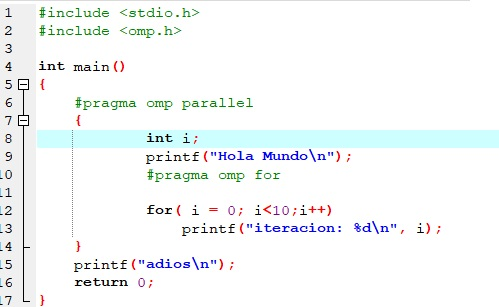
\includegraphics[scale=.8]{ejercicio7.jpg}


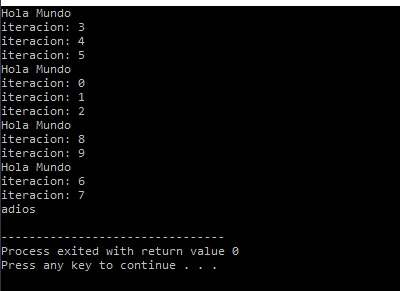
\includegraphics[scale=1]{ejercicio71.jpg}

Se puede observar que al repartirse las iteraciones del for entre los hilos,no todos realizan el mismo procedimiento, mostrando que algunos tienen mas carga de operaciones que otros.


\subsubsection*{Actividad 8}

Realiza la suma de dos arreglos unidimensionales de n elementos de forma paralela, utilizando los hilos por defecto que se generen en la region paralela y el constructor for.

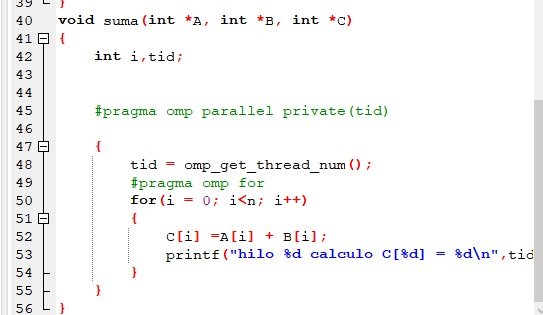
\includegraphics[scale=.8]{ejercicio8.jpg}


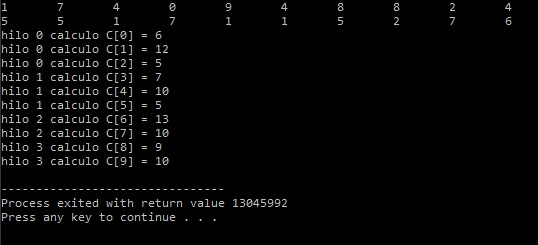
\includegraphics[scale=1]{ejercicio81.jpg}

Al utilizar dos regiones paralelas dentro del programa se puede observar que se generaron mas hilos, los primeros dos se generaron por la primera región paralela como en los ejercicios anteriores, y otros dos hilos se generaron para la región paralela del ciclo for.


\section{Conclusiones}

\subsubsection*{Mejía Alba Israel Hipólito }

Realizar esta práctica fue de gran provecho ya que ahora se pudo ver de una manera menos conceptual como es que se crean los programas en paralelo y se aprendió desde cero como usar OpenMP, cabe destacar que nos fue de gran ayuda las instrucciones del profesor para configurar Dev-C++ para poder correr las directivas de esta herramienta. El ejercicio de la práctica que más me llamo la atención fue el numero 3 el cual se pudo ver como al declarar una variable fuera de la paralelización y al momento de usarla en el código dentro esta, cada hilo comparte la misma variable, sin embargo, los valores que le da en ejecución son únicos en durante su proceso y cambia cuando se pasa a otro hilo. Este suceso se puede comparar también con el de la actividad 4 la cual se usa la cláusula prívate(i) la cual nos dice que a la variable i se le hará una copia por cada hilo que la use, la cual será eliminada después de que el programa se acabe de ejecutar.


\subsubsection*{Rosario Morales Oscar Daniel }

Al finalizar esta practica pudimos entender de mejor manera aunque básica, el funcionamiento de C en programas paralelos, a través de la clausula de \textit{pragma.omp.parallel} y \textit{pragma.omp.for},  donde la primera es para paralelizar cierta parte del código automáticamente, con la condición de considerar variables privadas o compartidas y el segundo para dividir el trabajo de un ciclo de repetición for, a través de realizar las mismas operaciones sobre distintos datos que no son dependientes entre si. Al principio se tuvo un poco de complicación al utilizar OpenMp ya que se trato de realizar en un entorno de Linux Ubuntu, pero consultando con el profesor, se comento la forma de realizar los programas en un IDE en windows, modificando las opciones de compilación del mismo. 







\end{document}